\subsection{Legacy Watcher}
\label{LegacyWatcher}

The legacy watcher is the standard (for now) watcher system GUI. It is written in OpenGL, wrapped in a creamy Qt shell. 

{\it legacyWatcher} source code can be found in {\tt .\slash src\slash clients\slash legacyWatcher}. The binary produced after building is 
named {\tt watcher}. 

\begin{figure}[htb]
\centering
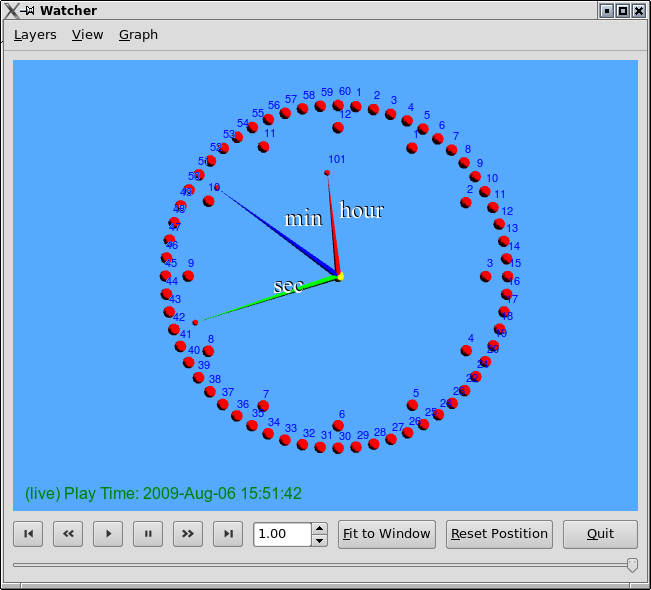
\includegraphics[width=0.8\textwidth]{legWatcherGUI.eps}
\caption{The legacy watcher showing a running instance of showClock.}
\label{fig:LegacyWatcherClock}
\end{figure}

\subsubsection{Command Line Options}
\begin{itemize}
\item {\tt -h} or {\tt --help}, show a usage message and exit. 
\item {\tt -f} of {--configFile}, gives the location of the configuration file. If not given a default one will be created, used, and saved on program exit.
\end{itemize}

\subsubsection{Configuration}
\begin{itemize}
\item {\tt server}, name or ipaddress of the server to connect to.
\item {\tt service}, name of service (usaully "watcherd") or port number on which the server is listening.
\item {\tt layers}, a listing of layers from the Layers menu. All layers the watcher knows about will show up here in a {\tt layername = bool} pair. 
If the bool is {\tt true}, the layer will be active (and shown), if {\tt false} the layer will not be shown. Every {\tt layername} will become
an entry in the {\tt layers} menu in the GUI.
\item {\tt nodes3d = bool}, if {\tt boolval} is {\tt true}, the GUI will use 3d shapes to diplay the MANET elements, otherwise 2d shapes will be used.
\item {\tt monochrome = bool}, if {\tt bool} is true all GUI elements in the main window will be black and white. Otherwise colors will be used. 
\item {\tt displayBackgroundImage = bool}, if {\tt bool} is true and a background image file is given, the background will be displayed. Otherwise it will not.
\item {\tt showVerboseStatusString = false}, if {\tt true} show extra debugging information in the status string in the main window.
\item {\tt showWallTime = true}, if {\tt true} show the current system time in the status string in the main window.
\item {\tt showPlaybackTime = true}, if {\tt true} show the current playback time (when the events happened) in the status string in the main window.
\item {\tt showPlaybackRange = true}, if {\tt true} show total time range (first event, last event) of playback in the status string in the main window.
\item {\tt statusFontName = ``name''}, the font name of the status string in the main window. e.g. ``Helvetica''. 
\item {\tt scaleText = float}, how much to scale the text in the main window.
\item {\tt scaleLine = float}, how much to scale lines in the main window.
\item {\tt layerPadding = float}, how much padding (in pixels) to place between layers. 
\item {\tt gpsScale = float}, a constant to multiply GPS coordinates against.
\item {\tt antennaRadius = float}, how big the ``antenna radius'' is in meters (for display only - does not effect connectivity). 
\item {\tt ghostLayerTransparency = float}, how transparent to make the ``ghost layer'', when layers are spread more than a few pixels apart.
\item {\tt statusFontPointSize = float}, the font size of the status string. 
\item {\tt backgroundImage:imageFile=filename}, the location of the background image to use, or ``none'' (with quotes) if not using a background image.
\item {\tt backgroundImage:coordinates = [ x, width, y, height]}, the initial location of the background image. This can be adjusted manually by using the right mouse button, while holding the shift key.
\item {\tt viewPoint : angle = [x, y, z]}, the initial angle of the main window view point with respect to the MANET.
\item {\tt viewPoint : scale = [x, y, z]}, the initial scale of the main window view point with respect to the MANET.
\item {\tt viewPoint : shift = [x, y, z]}, the initial shift of the main window view point with respect to the MANET.
\item {\tt backgroundColor : r=float}, the {\it red} component of the background color expressed as number between 0 and 1.
\item {\tt backgroundColor : g=float}, the {\it green} component of the background color expressed as number between 0 and 1.
\item {\tt backgroundColor : b=float}, the {\it blue} component of the background color expressed as number between 0 and 1.
\item {\tt backgroundColor : a=float}, the {\it alpha} component of the background color expressed as number between 0 and 1.
\end{itemize}

\subsubsection{User Interface}
The user interface for the watcher consists of a main window which displays the MANET, playback controls, a few buttons, and three pull down menus.

The main window is the heart of the visualization of the MANET. It is here where all the nodes, connections, labels, and layers are displayed. The 
user can use interact with the main window via the mouse or keyboard shortcuts. Mouse usage and keyboard shortcuts are given below.

\subsubsection{Layer Menu}
\begin{figure}[htb]
\centering
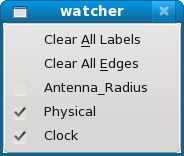
\includegraphics[width=0.2\textwidth]{legWatcherLayersMenu.eps}
\caption{An instance of the layer menu in the watcher GUI. Layers appear here dynamically.}
\label{fig:legWatcherLayersMenu}
\end{figure}

\subsubsection{View Menu}
\begin{figure}[htb]
\centering
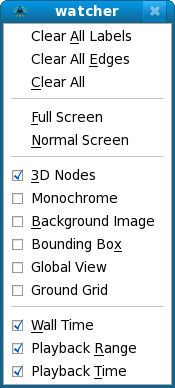
\includegraphics[width=0.2\textwidth]{legWatcherViewMenu.eps}
\caption{The view menu in the watcher GUI.}
\label{fig:legWatcherViewMenu}
\end{figure}

\subsubsection{Graph Menu}



